\documentclass{report}

\input{../template/preamble}
\input{../template/macros}
\input{../template/letterfonts}

\usetikzlibrary{graphs}

\title{\Huge{Electro Technique}\\Semester 5}
\author{\huge{Ahmad Abu Zainab}}
\date{}

\begin{document}

\maketitle
\newpage% or \cleardoublepage
% \pdfbookmark[<level>]{<title>}{<dest>}
\pdfbookmark[section]{\contentsname}{toc}
\tableofcontents
\pagebreak


\chapter{Polyphase Systems}

A polyphase system is a set of the same sinusoidal quantities (voltages or currents), of the same frequency and out of phase with respect to each other.

\begin{align*}
	v_1                & = A_1\sin \omega t + \varphi_1                   \\
	v_2                & = A_2\sin \omega t + \varphi_2                   \\
	\MTFlushSpaceBelow & \shortvdotswithin{=}          \MTFlushSpaceAbove \\
	v_m                & = A_m\sin \omega t + \varphi_m
\end{align*}

Such a system is referred to as balanced if

\begin{enumerate}
	\ii The effective values are equal
	\[
		A_1 = A_2 = \cdots = A_m
		.\]
	\ii The phase shift between each 2 consecutive
	\[
		\Delta \varphi = k \frac{2\pi }{m}
		.\]
	where $ m $ is the number of phases and $ k  $ is the order of succession separating 2 successive numbers.

\end{enumerate}

\begin{figure}[H]
	\centering
	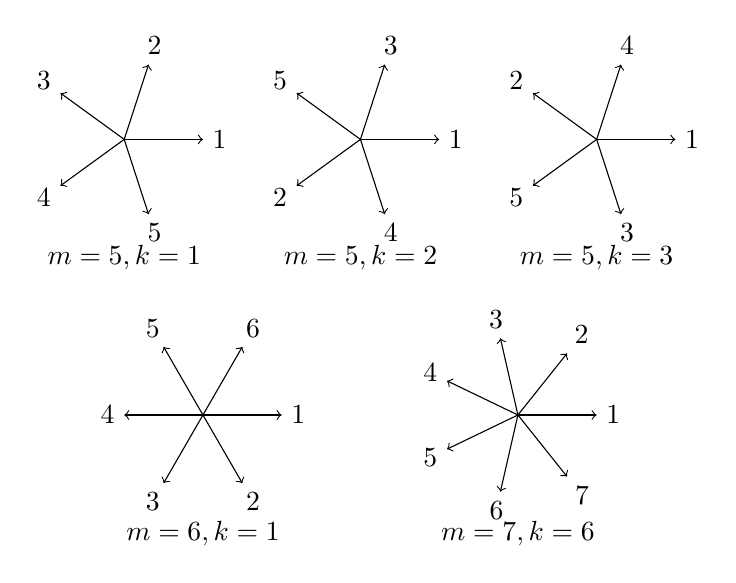
\begin{tikzpicture}
		\begin{scope}[xshift=-3cm]
			\foreach \angle in {5,...,1} {
					\draw[->] (0,0) -- ({(\angle-1)*360/5}:1) node[pos=1, anchor=180+(\angle-1)*360/5] {\angle};
				}
			\draw (0,-1.5) node {$m=5, k=1$};
		\end{scope}
		\begin{scope}[xshift=0cm]
			\foreach \angle in {1,...,5} {
					\draw[->] (0,0) -- ({-2*(\angle-1)*360/5}:1) node[pos=1, anchor=180-2*(\angle-1)*360/5] {\angle};
				}
			\draw (0,-1.5) node {$m=5, k=2$};
		\end{scope}
		\begin{scope}[xshift=3cm]
			\foreach \angle in {1,...,5} {
					\draw[->] (0,0) -- ({-3*(\angle-1)*360/5}:1) node[pos=1, anchor=180-3*(\angle-1)*360/5] {\angle};
				}
			\draw (0,-1.5) node {$m=5, k=3$};
		\end{scope}
		\begin{scope}[xshift=-2cm,yshift=-3.5cm]
			\foreach \angle in {1,...,6} {
					\draw[->] (0,0) -- ({-1*(\angle-1)*360/6}:1) node[pos=1, anchor=180-1*(\angle-1)*360/6] {\angle};
				}
			\draw (0,-1.5) node {$m=6, k=1$};
		\end{scope}
		\begin{scope}[xshift=2cm,yshift=-3.5cm]
			\foreach \angle in {1,2,...,7} {
					\draw[->] (0,0) -- ({-6*(\angle-1)*360/7}:1) node[pos=1, anchor=180-6*(\angle-1)*360/7] {\angle};
				}
			\draw (0,-1.5) node {$m=7, k=6$};
		\end{scope}
	\end{tikzpicture}
\end{figure}

\section{Production of a polyphase system}

Consider a uniform magnetic field $\va{B}$ going in the right direction, then consider a metal rod $S_1$ rotating at an angle $(\va{B},S_1) = \omega t + \varphi_0$. The rod will generate an emf of equation $ e_1(t) = E_m \sin \omega t + \varphi_0 $. We can insert new rods $S_2,S_3,\ldots,S_n$ each at an angle $(\va{B},S_i) = \omega t + \varphi_i$ which results in a polyphase emf.


\begin{minipage}{0.5\textwidth}
	\begin{align*}
		e_1(t) & = E_m\sin \omega t                            \\
		e_2(t) & = E_m\sin \omega t - \frac{2 \pi }{m}         \\
		e_3(t) & = E_m\sin \omega t - 2\cdot\frac{2 \pi }{m}   \\
		       & \vdotswithin{=}                               \\
		e_m(t) & = E_m\sin \omega t - (m-1)\cdot\frac{2\pi}{m} \\
	\end{align*}

\end{minipage}
\hfill
\begin{minipage}{0.5\textwidth}
	\begin{align*}
		\dot{e}(t) & = E_m\phase{0}                      \\
		\dot{e}(t) & = E_m\phase{-\frac{2 \pi }{m}}      \\
		\dot{e}(t) & = E_m\phase{-2\frac{2 \pi }{m}}     \\
		           & \vdotswithin{=}                     \\
		\dot{e}(t) & = E_m\phase{-(m-1)\frac{2 \pi }{m}} \\
	\end{align*}
\end{minipage}


\begin{figure}[H]
	\centering
	\ctikzset{bipoles/length=1cm}
	\begin{circuitikz}
		\begin{scope}[scale=0.75]
			\begin{scope}
				\draw (3,0) to[short] (0,0) to[L, l=$e_m$] (0,1.5) to[short] (3,1.5) to[european resistor, l=$Z_m$] (3,0);
			\end{scope}
			\begin{scope}[yshift=2cm]
				\draw[dashed] (0,0) to[short] (0,1);
			\end{scope}
			\begin{scope}[yshift=3.5cm]
				\draw (3,0) to[short] (0,0) to[L, l=$e_2$] (0,1.5) to[short] (3,1.5) to[european resistor, l=$Z_2$] (3,0);
			\end{scope}
			\begin{scope}[yshift=5.5cm]
				\draw (3,0) to[short] (0,0) to[L, l=$e_1$] (0,1.5) to[short] (3,1.5) to[european resistor, l=$Z_1$] (3,0);
			\end{scope}
		\end{scope}
	\end{circuitikz}
\end{figure}


\begin{figure}[H]
	\centering
	\ctikzset{bipoles/length=1.2cm}
	\begin{circuitikz}
		\begin{scope}[scale=0.75]
			\draw (0,0.5) to[short] (1,2) to[L,l=$e_1$, i=$i_1$] (3,2) to[short] (13,2) to[european resistor,l=$Z_1$] (13,-3.5);
			\draw (0,0.5) to[short] (1,1) to[L,l=$e_2$, i=$i_2$] (3,1) to[short] (11.5,1) to[european resistor,l=$Z_2$] (11.5,-3.5);
			\draw[densely dashed] (0,0.5) to[short] (1,0) to[short] (3,0) to[short] (10,0) to[short] (10,-3.5);
			\draw (0,0.5) to[short] (1,-1) to[L,l=$e_n$, i=$i_n$] (3,-1) to[short] (8.5,-1) to[european resistor,l=$Z_n$] (8.5,-3.5);

			\draw (13,-3.5) to[short] (5.5,-3.5) to[short, i=$i_N$] (0,-3.5) to[short,-*] (0,0.5);

			\draw[thin, ->, red] (4,1) -- (4,2) node[pos=0.5, anchor=west] {$U_{12}$};
			\draw[thin, ->, red] (4,0) -- (4,1) node[pos=0.5, anchor=west] {$U_{23}$};
			\draw[thin, ->, red] (4,-1) -- (4,0) node[pos=0.5, anchor=west] {$U_{n-1\,n}$};
			\draw[thin, ->, red] (3.5,2) -- (3.5,-1) node[pos=0.5, anchor=east] {$U_{n1}$};

			\draw[thin, ->, blue] (6,-3.5) -- (6,2) node[pos=1, anchor=south] {$V_1$};
			\draw[thin, ->, blue] (6.5,-3.5) -- (6.5,1) node[pos=1, anchor=south] {$V_2$};
			\draw[thin, ->, blue] (7,-3.5) -- (7,-1) node[pos=1, anchor=south] {$V_n$};

			\draw (0,0.5) to[short,-*] (0,0.5) node[anchor=east] {$N$};
		\end{scope}
	\end{circuitikz}
\end{figure}

\begin{figure}[H]
	\centering
	\ctikzset{bipoles/length=1.2cm}
	\begin{circuitikz}
		\begin{scope}[scale=0.75]
			\draw[thin, ->, red] (4,1) -- (4,2) node[pos=0.5, anchor=west] {$U_{12}$};
			\draw[thin, ->, red] (4,0) -- (4,1) node[pos=0.5, anchor=west] {$U_{23}$};
			\draw[thin, ->, red] (4,-1) -- (4,0) node[pos=0.5, anchor=west] {$U_{n-1\,n}$};
			\draw[thin, ->, red] (3.5,2) -- (3.5,-1) node[pos=0.5, anchor=east] {$U_{n1}$};

			\draw[thin, ->, blue] (6,-4.25) -- (6,2) node[pos=1, anchor=south] {$V_1$};
			\draw[thin, ->, blue] (6.5,-4.25) -- (6.5,1) node[pos=1, anchor=south] {$V_2$};
			\draw[thin, ->, blue] (7,-4.25) -- (7,-1) node[pos=1, anchor=south] {$V_n$};

			\draw[thin, blue] (10.75,-4.25) -- (6,-4.25);

			\draw (0,0.5) to[short] (1,2) to[L,l=$e_1$, i=$i_1$] (3,2) to[short] (13,2) to[european resistor,l=$Z_1$] (13,-3.5) to[short] (10.75,-4.25) node[anchor=north] {$N'$};
			\draw (0,0.5) to[short] (1,1) to[L,l=$e_2$, i=$i_2$] (3,1) to[short] (11.5,1) to[european resistor,l=$Z_2$] (11.5,-3.5) to[short] (10.75,-4.25);
			\draw[densely dashed] (0,0.5) to[short] (1,0) to[short] (3,0) to[short] (10,0) to[short] (10,-3.5) to[short] (10.75,-4.25);
			\draw (0,0.5) to[short] (1,-1) to[L,l=$e_n$, i=$i_n$] (3,-1) to[short] (8.5,-1) to[european resistor,l=$Z_n$] (8.5,-3.5) to[short, -*] (10.75,-4.25);

			\draw (0,0.5) to[short,-*] (0,0.5) node[anchor=east] {$N$};
		\end{scope}
	\end{circuitikz}
\end{figure}

In the course (and in real life) we almost always study three phase systems. As such, we obtain the following

\begin{minipage}[t]{0.5\linewidth}
	\begin{align*}
		V_1 & = V \phase{\ang{0}}    \\
		V_2 & = V \phase{\ang{-120}} \\
		V_3 & = V \phase{\ang{120}}
	\end{align*}

	\begin{align*}
		I_1 & = J_{12} - J_{31} \\
		I_2 & = J_{23} - J_{12} \\
		I_3 & = J_{31} - J_{23}
	\end{align*}

\end{minipage}
\hfill
\begin{minipage}[t]{0.5\linewidth}
	\begin{align*}
		U_{12} & = V_1 - V_2 = U \phase{\ang{30}}  \\
		U_{23} & = V_2 - V_3 = U \phase{\ang{-90}} \\
		U_{31} & = V_3 - V_1 = U \phase{\ang{150}}
	\end{align*}
	\begin{align*}
		J_{12} & = \frac{U_{12}}{Z_{12}} \\
		J_{23} & = \frac{U_{23}}{Z_{23}} \\
		J_{31} & = \frac{U_{31}}{Z_{31}}
	\end{align*}
\end{minipage}
\begin{align*}
	U & = \sqrt{3} V \\
	I & = \sqrt{3} J
\end{align*}

Given a $\Delta$ configuration, we can calculate the currents in each branch by (regardless of if the system is balanced or not)

\begin{figure}[H]
	\centering
	% \begin{tikzpicture}
	% 	\graph { $V$ -> $U$ -> $J$ -> $I$ };
	% \end{tikzpicture}
	\begin{tikzpicture}[ nodes = {text depth = 1ex, text height = 2ex}]
		\graph { V/$V$ -> U/$U$ -> J/$J$ -> I/$I$ };
	\end{tikzpicture}
\end{figure}

To find the voltages in an unbalanced Y configuration, we calculate the following quantity (Millman's Method)
\[
	V_0 = \frac{V_{S1}Y_1 + V_{S2}Y_2 + V_{S3}Y_3}{Y_1 + Y_2 + Y_3 + Y_N}
	.\]

Where

\[
	Y_n = \frac{1}{Z_n}
	.\]

\begin{align*}
	V_1 & = V_{S1} - V_0 \\
	V_2 & = V_{S2} - V_0 \\
	V_3 & = V_{S3} - V_0
\end{align*}

\section{Power in Triphase systems}

\begin{align*}
	P & = V_1I_1\cos \varphi_1 + V_3I_3\cos \varphi_2 + V_3I_3\cos \varphi_3 \\
	Q & = V_1I_1\sin \varphi_1 + V_3I_3\sin \varphi_2 + V_3I_3\sin \varphi_3 \\
	S & = V_1I_1^* + V_3I_3^* + V_3I_3^*
\end{align*}

If the load is symmetric

\begin{align*}
	P & = 3VI \cos \varphi = \sqrt{3}UI \cos \varphi \\
	Q & = 3VI \sin \varphi = \sqrt{3}UI \sin \varphi \\
	S & = 3VI^* = \sqrt{3}UI^*
\end{align*}

\chapter{Magnetic Circuits}

We characterise a magnetic field by 2 vectors: the magnetic field density (induction) $\va{B}\; [\unit{\tesla}]$ and the magnetic field intensity (field) $\va{H}\; [\unit{\ampere\per\metre}]$

\[
	\va{B}= \mu_0 \va{H}
	.\]

where $\mu_0$ is the magnetic permeability $[\unit{\henry\per\metre}]$. \\

The set of magnetic lines crossing a surface is called magnetic flux

\[
	\Phi = \va{B}\cdot\va{S}
	.\]

Ampere's law:
\[
	\underbrace{\oint_{(f)} H \dd{\ell}}_{\substack{\text{circulation of}\\ \text{the magentic field}}}
	=
	\underbrace{\sum i = ni}_{\mathclap{\substack{\text{total current}\\ \text{ignited by}\\ \text{the contour}}}}
	.\]

Biot–Savart law

\[
	\dd{H} = \frac{i}{4\pi} \frac{\dd{\ell}\sin \alpha}{r^2}
	.\]

Some values of $H$ for specific cases
\begin{align*}
	\text{Infinite wire: } & H = \frac{i}{2\pi r}                                 \\
	\text{Circular wire: } & H = \frac{i}{2 r}                                    \\
	\text{Solenoid: }      & H = \frac{ni}{2\ell} (\cos \theta_1 + \cos \theta_2) \\
	                       & H_\text{center} = \frac{ni}{\ell} \cos \theta        \\
	\text{Flat coil: }     & H = \frac{ni}{2r}
\end{align*}

\section{Magnetic Substances}

\subsection{Magnetic Permeability $\mu$}

Magnetic permeability of most substances are very close to $\mu_0$ and practically constant
\[
	\mu_0 = 4\pi\times 10^{-7} \; [\unit{\henry\per\metre}]
	.\]

While some materials like metals have a much higher permeability, and are called ferromagnetic materials. The permeability of these materials is not constant and depends on the magnetic field intensity $H$.

Substances are classified into 2 categories
\begin{enumerate}
	\ii Non-magnetic substances: diamagnetic and paramagnetic substances.
	\ii Magnetic substances: ferromagnetic substances.
\end{enumerate}

\subsection{Diamagnetic and Paramagnetic Substances}

We define the magnetic susceptibility $\chi$ as
\[
	\chi = \mu_r -1
	.\]

\begin{itemize}
	\ii Vacuum: $\chi = 0$ ($\mu_r=1$).
	\ii Diamagnetic substances: $\mu_r>1\Rightarrow\chi < 0$.
	\ii Paramagnetic substances: $\mu_r<1\Rightarrow\chi > 0$.
\end{itemize}

\subsection{Ferromagnetic Substances}

These substances are able to concentrate the magnetic flux in their volume. Their $\mu$ is very large.

\subsection{Influence of Temperature}

Paramagnetic and Ferromagnetic substances have a $\chi$ depends on $T$. As $T$ increases, $\chi$ decreases until it reaches a critical temperature (Curie point) $T_c$ where $\chi = 0$ and the substance becomes paramagnetic.

\begin{figure}[H]
	\centering
	\begin{tikzpicture}[
			declare function={
					% arcsinh
					arcsinh(\x) = ln(\x + sqrt(\x^2+1));
					% magnetization
					m(\x) = and(\x>=0,\x<1) * (1 - (sinh(arcsinh(1)/x))^(-4))^(1/8) + or(\x<0,\x>=1) * (0);
				}]

		\begin{axis}[
				xlabel = {$T/T_c$},
				ylabel = {$\chi$},
				smooth,thick,
				domain=0:1.8,
				ymax=1.6,
				axis lines = center,
				every tick/.style = {thick}]

			\addplot[color=blue,very thick,samples=300]{m(x)};
		\end{axis}
	\end{tikzpicture}
\end{figure}


\section{Magnetic Circuits}

A magnetic circuit is a closed path in which a magnetic flux is concentrated. It is made of a ferromagnetic core and a coil. The coil is used to create a magnetic field in the core.

\subsection{Properties of Magnetic Circuits}

The flux is the same in all parts of the circuit.

\[
	\Phi = \va{B}\cdot\va{S} = B \cdot S \cdot \cos \alpha
	.\]

The exciter coil is characterised by the number of turns $n$ and the current $i$.

\[
	\SF = ni\;[\unit{\ampere t}]
	.\]

\begin{align*}
	\text{Electric Circuit}                & \rightarrow \text{Magnetic Circuit}                               \\
	I\;[\unit{\ampere}]                    & \rightarrow \Phi\;[\unit{\weber}]                                 \\
	E\;[\unit{\volt}]                      & \rightarrow \SF\;[\unit{\ampere}]                                 \\
	R = \frac{l}{\sigma S}\; [\unit{\ohm}] & \rightarrow \mcR = \frac{l}{\mu S} \; [\unit{\ampere \per\weber}]
\end{align*}

\thm{Hopkinson's Law}{
	The sum of the magnetic forces in a magnetic circuit is equal to the sum of the magnetomotive forces.

	\[
		\SF = \sum \SF_i = \mcR \Phi
		.\]

}

\dfn{Magnetic Potential Difference}{
	The magnetic potential difference between 2 points (A and B) of a magnetic circuit is the work needed to move a unit magnetic pole from one point to the other.

	\[
		\theta_\text{AB} = \Phi \mcR_\text{AB}
		.\]

	such that
	\[
		\mcR_\text{AB} = \ell_\text{AB} H
		.\]
}

\thm{Ampere's Law}{
	The circulation of the magnetic field intensity in a magnetic circuit is equal to the sum of the currents in the circuit.

	\[
		\oint_{\cramped{(f)}} H \dd{\ell} = \sum n_i I_i = \sum \SF_i = \SF
		.\]

	In case of a constant cross section, we have
	\[
		H = \frac{\SF}{\ell}
		.\]
}

\section{Non-Homogeneous Magnetic Circuits}

A non-homogeneous magnetic circuit is a magnetic circuit built with different materials.\\

Let 1 and 2 be two materials with different permeabilities $\mu_1$ and $\mu_2$, and assume that the circuit is not saturated($B(H)$ is linear).\\

\begin{align*}
	\Phi_1        & = \Phi_2        \\
	B_1 S_1       & = B_2 S_2       \\
	\mu_1 H_1 S_1 & = \mu_2 H_2 S_2 \\
\end{align*}

\[
	\sum \SF_i = H_1 \ell_1 + H_2 \ell_2
	.\]

\begin{align*}
	H_1 & = \frac{\sum \SF_i}{\ell_1 + \ell_2 \frac{\mu_1}{\mu_2} \frac{S_1}{S_2}} \\
	H_2 & = \frac{\sum \SF_i}{\ell_1 \frac{\mu_2}{\mu_1} \frac{S_2}{S_1} + \ell_2}
\end{align*}

\[
	\sum \SF_i = \Phi(\mcR_1 + \mcR_2) = \Phi \lt( \frac{\ell_1}{\mu_1 S_1} + \frac{\ell_2}{\mu_2 S_2} \rt)
	.\]

\section{Self-Inductance of a coil}

Consider a magentic circuit excited by a coil of $n$ turns, the circuit is then traversed by a flux $\Phi$. We define $\Psi$ as the flux linked to a single turn of the coil.

\[
	\Psi = n \Phi = n\frac{\SF}{\mcR} = \frac{n^2}{\mcR} I
	.\]

We define the self-inductance of the coil as

\[
	L = \frac{\Psi}{I} = \frac{n^2}{\mcR}
	.\]

\nt{
	In an non-saturated magnetic circuit, the self-inductance of a coil is constant.
}

\section{Energy of a Magnetic Circuit}

Here we assume that the magnetic circuit is non-saturated ($B(H)$ is linear), no leakage flux, and the exciter coil has negligible resistance.\\

Coil has a constant inductance $L=\frac{n^2}{\mcR}$. Assume all the energy is transferred to the magnetic circuit.

\[
	\dd{W_e} = \dd{W_m} = H \ell S \dd{B} = H \tau \dd{B}
	.\]

where $\tau = \ell S$ is the volume of the magnetic circuit.

\[
	\dd{W'_m} = \frac{\dd{W_m}}{\tau} = H \dd{B}
	.\]

The total magnetic energy is

\begin{align*}
	W_m  & = \int Li \dd{i} = \frac{1}{2} Li^2 = \frac{1}{2} \Psi i \\
	W'_m & = \int H \dd{B} = \frac{1}{2} H B
\end{align*}

\section{Leakage Flux}

In a real magnetic circuit, the flux is not entirely concentrated in the core. Some of it leaks out of the core. If we assume that the leakage flux is not negligible then the flux is equal at all points of the circuit.

\[
	\Phi = \underbrace{\Phi_m}_{\text{main flux}} + \underbrace{\Phi_f}_{\text{leakage flux}}
	.\]

\thm{Hopkinson's Law and leakage flux}{
	\[
		L_m = \frac{n\Phi_m}{I} = \frac{\Psi_m}{I} = \frac{n^2}{\mcR}
		.\]

	\[
		\Psi_f \propto I \implies \Psi_f = L_f I \implies L_f = \frac{\Psi_f}{I}
		.\]

	\[
		L = L_m + L_f
		.\]
}

We define Hopkinson's coefficient as

\[
	\upsilon = \frac{L}{L_m}
	.\]

\section{Mutual Inductance}

Consider 2 coils $C_1$ and $C_2$ linked within a magnetic circuit. The flux $\Phi_{21}$ created by $C_1$ at $C_2$.

\[
	\Psi_{21} = n_2 \Phi_{1} = L_{21} I_1 = M_2 I_1
	.\]

Similarly we can define $\Psi_{12}$ and $M_1$.

\[
	\Psi_{12} = n_1 \Phi_{2} = L_{12} I_2 = M_1 I_2
	.\]

\begin{align*}
	M_2 & = n_1 n_2 \frac{\mu S}{\ell} = \frac{n_1 n_2}{\mcR} \\
	M_1 & = n_1 n_2 \frac{\mu S}{\ell} = \frac{n_1 n_2}{\mcR}
\end{align*}

In an ideal circuit

\[
	M_1 = M_2 = M = \begin{cases}
		\sqrt{L_1 L_2}  & \text{if \(\Phi_1\) and \(\Phi_2\) have the same sense}     \\
		-\sqrt{L_1 L_2} & \text{if \(\Phi_1\) and \(\Phi_2\) have the opposite sense}
	\end{cases}
	.\]

\subsection{Case of non-ideal circuit}

Practically, in the case of leakage flux $M<\sqrt{L_1 L_2}$.

\[
	k = \frac{M}{\sqrt{L_1 L_2}}
	.\]

\[
	M = \sqrt{L_{m_1} L_{m_2}} \implies k = \frac{1}{\sqrt{\upsilon_1 \upsilon_2}}
	.\]

\section{Non-Linear}

In this case, the magnetic circuit is saturated. The flux is no longer proportional to the magnetomotive force.
\[
	\SF \neq \mcR \Phi \neq \sum H_i \ell_i
	.\]

\subsection{Partial Characteristics Method}

Knowing the curve $B(H)$, we can trace $\Phi(H\ell)$ by multiplying $B$ by the cross sectional $S$ and by multiplying $H$ by the length $\ell$.

\subsection{Series Magnetic Circuits}

\[
	\SF = H_1 \ell_1 + H_2 \ell_2 + \cdots + H_n \ell_n = \theta_1 + \theta_2 + \cdots + \theta_n
	.\]

\section{Series-Parallel Magnetic Circuits}

\[
	\Phi = \Phi_1 + \Phi_2
	.\]

\[
	\theta_1 = \theta_2 = H_1 \ell_1 = H_2 \ell_2 = \theta
	.\]
\end{document}
